\documentclass[]{article}

% Imported Packages
%------------------------------------------------------------------------------
\usepackage{amssymb}
\usepackage{amstext}
\usepackage{amsthm}
\usepackage{amsmath}
\usepackage{enumerate}
\usepackage{fancyhdr}
\usepackage[margin=1in]{geometry}
\usepackage{graphicx}
%\usepackage{extarrows}
%\usepackage{setspace}
%\usepackage{xcolor}
\usepackage{color}
%------------------------------------------------------------------------------

% Header and Footer
%------------------------------------------------------------------------------
\pagestyle{plain}  
\renewcommand\headrulewidth{0.4pt}                                      
\renewcommand\footrulewidth{0.4pt}                                    
%------------------------------------------------------------------------------

% Title Details
%------------------------------------------------------------------------------
\title{Deliverable \#1 Template : Software Requirement Specification (SRS)}
\author{SE 3A04: Software Design II -- Large System Design}
\date{\today}
                            
%------------------------------------------------------------------------------

% Document
%------------------------------------------------------------------------------
\begin{document}

\maketitle	
\noindent{\bf Tutorial Number:} T01\\
{\bf Group Number: G3} Gx \\
{\bf Group Members:} 
\begin{itemize}
	\item Group Member Name (as listed in Avenue)
	\item You do not need to use student \#s or macid (keep those private).
\end{itemize}

\section*{IMPORTANT NOTES}
\begin{itemize}
	\item Be sure to include all sections of the template in your document regardless whether you have something to write for each or not
	\begin{itemize}
		\item If you do not have anything to write in a section, indicate this by the \emph{N/A}, \emph{void}, \emph{none}, etc.
	\end{itemize}
	\item Uniquely number each of your requirements for easy identification and cross-referencing
	\item Highlight terms that are defined in Section~1.3 (\textbf{Definitions, Acronyms, and Abbreviations}) with \textbf{bold}, \emph{italic} or \underline{underline}
	\item For Deliverable 1, please highlight, in some fashion, all (you may have more than one) creative and innovative features. Your creative and innovative features will generally be described in Section~2.2 (\textbf{Product Functions}), but it will depend on the type of creative or innovative features you are including.
\end{itemize}

\newpage
\section{Introduction}
\label{sec:introduction}
% Begin Section
This SRS will describe the software requiremnets for GeoLens, a community-driven application for identifying
locations based on images, descriptitons and discussions. This document outlines the system's overall purpose, the context for building the application,
functional and non-functional requirements and user iteraction.

\subsection{Purpose}
\label{sub:purpose}
% Begin SubSection
This document serves as a guideline for developers, designers, QA engineers, project managers and other stakeholders, ensuring a clear understanding of the system, including it's objectives, users, expected behavior, and technical constraints.
As the project progresses and changes, the document will provide a baseline from which these changes can be compared. This SRS may also aid in risk identification early in the project lifecycle by outlining dependencies and constraints, allowing managers to prevent risks.
% End SubSection

\subsection{Scope}
\label{sub:scope}
% Begin SubSection
GeoLens is a community and AI driven application designed to identify locations from images. It consists of several individual software products described below.\\

The \textbf{Forum} UI is the primary interface where users interact with GeoLens. It allows users to upload images of locations for identification, view responses, and
engage with the community. If the forum UI can provide ease of use and an interactive experience it will encourage community engagement and bring traffic to the
application. The interface facilitates discussions, displays aggregated predictions, and contains gamification elements such as leaderboards. The forum UI should be accessible
to all users, intuitive to use and respond to user requests within 100 ms. It does not perform image analysis or identification itself but serves as the user’s gateway to the platform.\\

The \textbf{Orchestrator} is responsible for handling submitted images, delegating tasks to experts,
and returning the final result to users. The Orchestrator should coordinate system components concurrently, managing task distribution, monitoring progress, and aggregating responses to ensure quick and accurate results. It handles task prioritization, load balancing, and error recovery while maintaining seamless interactions between users and experts.
The back end does not analyze images directly but functions as the between layer that processes requests and returns items to the forum.\\

The \textbf{Host DBMS} stores user account information, historical user interactions, reputation scores, previously identified locations and leaderboards. It ensures that the system retains valuable data,
in a structured way that is efficiently accessible by other system components. The database should be highly secure, as it contains sensitive user information. The database does not process images or make
identifications but acts as the central location for all platform data. \\

The three \textbf{Experts} are as follows:
\begin{enumerate}
    \item \textbf{GeoKnowr AI}
    \begin{itemize}
        \item Pre-trained image processing model
        \item Predicts coordinates where an image was taken
    \end{itemize}
    \item \textbf{Landmark Recognition}
    \begin{itemize}
        \item Google images API
        \item Search by image to locate a popular landmark
    \end{itemize}
	\item \textbf{Region Specific AI}
	\begin{itemize}
        \item Uses a specialized AI model trained for a specific region
        \item Enhances accuracy for areas with distinct visual features
    \end{itemize}
\end{enumerate}

The primary goal of these experts is to work cohesively to provide an accurate prediction with little delay. GeoKnowr AI aims to deliver an initial estimate
of where an image was taken by assigning coordinates. Then the region specific AI can further refine this prediction by applying localized knowledge. If a landmark is 
present in the image, the Landmark Recognition software should pin point it's location.

\subsection{Definitions, Acronyms, and Abbreviations}
\label{sub:definitions_acronyms_and_abbreviations}
% Begin SubSection
\begin{itemize}
	\item \textbf{GeoLens:} the system being specified
	\item \textbf{AI:} Aritficial Intelligence
\end{itemize}
% End SubSection

\subsection{References}
\label{sub:references}
% Begin SubSection
\begin{itemize}
	\item Provide a complete list of all documents referenced elsewhere in the SRS.
	\item Identify each document by title, report number (if applicable), date, and publishing organization.
	\item Specify the sources from which the references can be obtained.
	\item Order this list in some sensible manner (alphabetical by author, or something else that makes more sense).
\end{itemize}
% End SubSection

\subsection{Overview}
\label{sub:overview}
% Begin SubSection
Section 2 aims to put the value of GeoLens into perspective, relating and contrasting it to other similar products that currently exist.
It should also provide a summary of the primary functions of the application and a description of the expected users. This should provide readers with a general understanding
of the system, and how users are expected to intereact with it. Finally, constraints and assumptions are listed to clarify the scope of the application and the context in which it operated.\\\\
Section 3 presents a use case digram outlining the main functionality and interactions with stakeholders.\\\\
Section 4 is a detailed overview of the functional requirements, discussing what the system will do. These requirements will be organized in terms of 
business events, viewpoints and scenarios. This provides a structured understanding of the system in various contexts. \\\\
Finally, section 5 describes the Non-Functional Requirements, focusing on how the system aims to be a valuable service. This section provides a rationale for each requirement, explaining their necessity and benefits.

% End Section

\section{Overall Product Description}
\label{sec:overall_description}
% Begin Section

% \begin{itemize}
% 	\item This section should describe the general factors that affect the product and its requirements. 
% 	\item It does not state specific requirements.
% 	\item It provides a \emph{background} for those requirements and makes them easier to understand.
% \end{itemize}


\subsection{Product Perspective}
\label{sub:product_perspective}
% Begin SubSection
\begin{itemize}
	% \item Put the product into perspective with other related products, i.e., context

	%This was bugging out my compiler
	%\noindent {AppName is a mobile game guessing app developed for the Android platform. A similar product is GeoGuessr, which allows users to guess the location of randomly given locations from a Google Street View. However, this product will require a user to submit a picture of a location they wish to identify. The application will consult the 3 experts: an algorithm that aggregates responses from users around the world, and AI model, and Rainbolt. Each expert will return a confidence level and if the confidence level meets a predefined threshold of 70\%, then that expert's response will be return in the same order as above. The product also consists of a unique feature, which is a game that has competition modes, where players can play against each other individually or as a group. Additionally, the product will allow users to create and modify profiles that will be used in the app. This means a login and signup feature will be required. The product will compare a photo taken by
	%}
	%\noindent {}

	\item If the product is independent and totally self-contained, it should be stated here
	\item If the SRS defines a product that is a component of a larger system, then this subsection should relate the requirements of that larger system to the functionality of the software being developed. Identify interfaces between that larger system and the software to be developed.
	\item A block diagram showing the major components of the larger system, interconnections, and external interfaces can be helpful
\end{itemize}
% End SubSection

\subsection{Product Functions}
\label{sub:product_functions}
% Begin SubSection
\begin{itemize}
	\item Provide a \emph{summary} of the major functions that the software will perform.
	\begin{itemize}
		\item \textbf{Example}: An SRS for an accounting program may use this part to address customer account maintenance, customer statement, and invoice preparation without mentioning the vast amount of detail that each of those functions requires.
	\end{itemize}
	\item Functions should be organized in a way that makes the list of functions understandable to the customer or to anyone else reading the document for the first time 
	\item Present the functions in a list format - each item should be one function, with a brief description of it
	\item Textual or graphical methods can be used to show the different functions and their relationships
	\begin{itemize}
		\item Such a diagram is not intended to show a design of a product, but simply shows the logical relationships among variables
	\end{itemize} 
\end{itemize}
% End SubSection

\subsection{User Characteristics}
\label{sub:user_characteristics}
% Begin SubSection
The app is meant to be a user-friendly app and as a result has the following expected qualifications of its users:\\ \\
1. Education Level: Basic Literacy and Geographical knowledge
\begin{itemize}
	\item A person with basic literacy skills of reading and writing should be able to utilize
		this app without any difficulties.
	\item A person with basic geographical knowledge of the divison of the world into continents, countries, and regions
		should be able to utilize this app without any difficulties.
\end{itemize}
2. Experience: Any
\begin{itemize}
	\item Since the app is meant to be user-friendly, someone who is using the app for the very first time
		should be able to do so without any major problems.
\end{itemize}
3. Technical Expertise: Basic knowledge of smartphone usage
\begin{itemize}
	\item A person having basic experience with the usage of a smartphone should be able to easily use the app.
\end{itemize}

% End SubSection

\subsection{Constraints}
\label{sub:constraints} \medskip
% Begin SubSection
1. \textbf{Budget: }The budget allocated to the project will have a great affect on which technologies may be used
in the development of the app, as well as limiting the external integrations that can be used. The indicated
budget for the project is \$0.\medskip \\
2. \textbf{Time: }The time allotted for the project with have a significant affect on the feasible scope of the
project. Consequently, this limits the number and quality of features that can be integrated into the app.
% End SubSection

\subsection{Assumptions and Dependencies}
\label{sub:assumptions_and_dependencies}
% Begin SubSection
1. Assume that pictures of locations will be able to be located to at minimum country level accuracy.\\
2. Assume that users encounter pictures of unknown origin (no information about where it was taken).\\
3. Assume that users wish to know where pictures of unknown origin were taken.\\
4. Assume that the processing of unauthorized photos of public spaces are legal in all regions in which the app operates. \medskip \\
Other assumptions that, if it fails to hold, could require a change to the requirements:\\
1. A recent (released within 3 years) version of the Andriod operating system will be available on the device.\\
2. The device will have internet access if the user wishes to use the app.\\
3. The app will have access to an on-device photo library if the user wishes to upload a photo.\\
4. Assume all API dependencies are fully functional during the operation of the product.
%\begin{itemize}
%	\item List any assumptions you made in interpreting what the software being developed is aiming to achieve
%	\item List any other assumptions you made that, if it fails to hold, could require you to change the requirements
	%\item List each of the factors that affect the requirements stated in the SRS
	%\item These factors are not design constraints on the software but are, rather, any changes to them that can affect the requirements in the SRS
%	\begin{itemize}
%		\item \textbf{Example}: An assumption may be that a specific operating system will be available on the hardware designated for the software product. If, in fact, the operating system is not available, the SRS would then have to change accordingly.
%	\end{itemize}
%\end{itemize}
% End SubSection

\subsection{Apportioning of Requirements}
\label{sub:apportioning_of_requirements}
% Begin SubSection
1. Further language capabilities
\begin{itemize}
	\item The software will be developed only in English for the first version
		of the system.
\end{itemize}
2. User rating/rank based on guess accuracy
\begin{itemize}
	\item Users will be able to guess on other user's posts as to where
		they think it is (This does \textbf{not} affect the expert determination
		and is simply to add game-like mechanics). In a future version of the software,
		each user will have a rating/rank
		based on how close their guesses are to the expert determination.
\end{itemize}
3. No question limit for paid tier
\begin{itemize}
	\item In a future version of the software, users would be able to
		purchase a paid premium tier to be able to ask as many questions
		per day as they'd like.
\end{itemize}
%\begin{itemize}
%	\item Identify requirements that may be delayed until future versions of the system
%\end{itemize}
% End SubSection

% End Section
\section{Use Case Diagram}
\label{sec:use_case_diagram}
% Begin Section
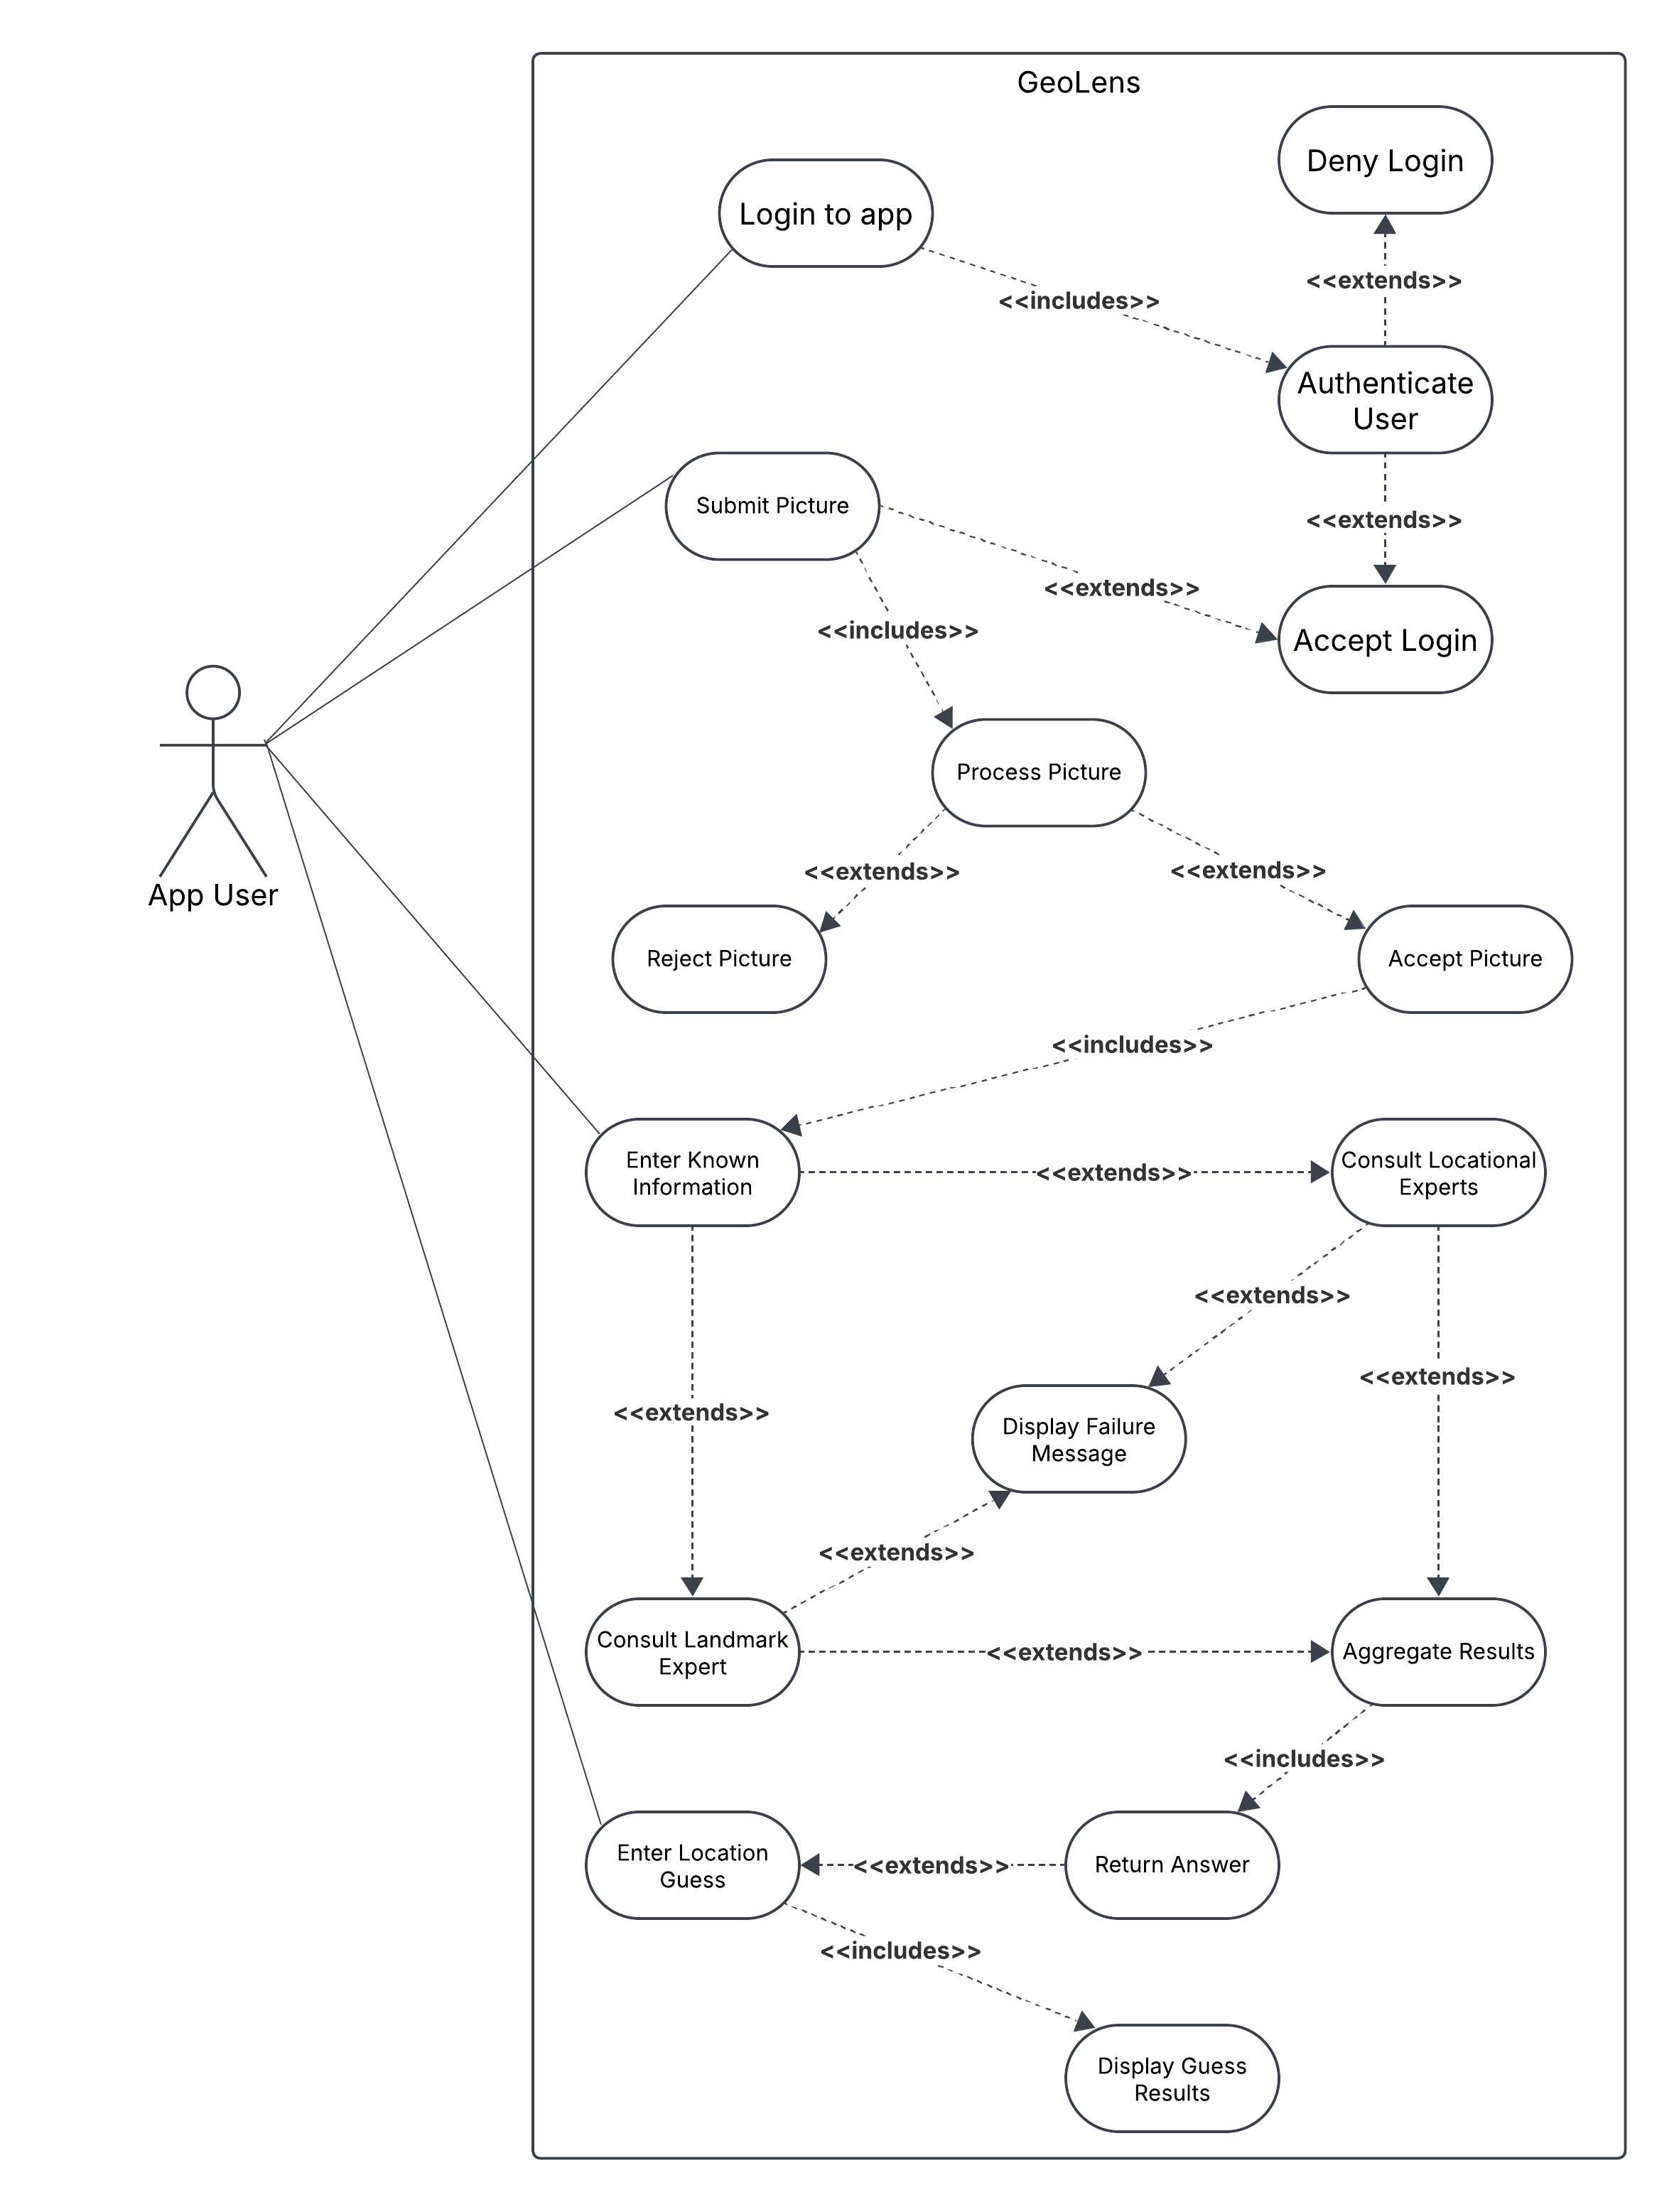
\includegraphics[scale=0.8]{usecase}
%\begin{itemize}
%	\item Provide the use case diagram for the system being developed.
%	\item You do not need to provide the textual description of any of the use cases here (these will be specified under "Highlights of Functional Requirements").
%	\item Provide \emph{one} use case diagram for the most important Business Event.
%	\item The text of all use cases will be specified under "Highlights of Functional Requirements"
%\end{itemize}
%In this section, select the most important Business Event that your system responds to and give its use case diagram.  Only one use case diagram is needed.  Give a brief textual description of the use case without repeating what is in the scenarios of the corresponding Business Event.

%
%
%
%This section should provide a use case diagram for your application. 
%\begin{enumerate}[a)]
%	\item Each use case appearing in the diagram should be accompanied by a text description. 
%\end{enumerate}
%% End Section

\section{Highlights of Functional Requirements}
\label{sec:functional_requirements}
% Begin Section
\begin{itemize}
	\item Specify all use cases (or other scenarios triggered by other events), organized by Business Event. 
	\item For each Business Event, show the scenario from every Viewpoint. You should have the same set of Viewpoints across all Business Events. If a Viewpoint doesn't participate, write N/A so we know you considered it still. You can choose how to present this - keep in mind it should be easy to follow. 
	\item At the end, combine them all into a Global Scenario.
	%\item Specify the "use cases" (or other triggering events) organized by Business Event. (The Global Scenario is what you might think of as a use case). Be sure to consider Business Events that aren't just triggered by users with goals (e.g. something happens in the environment that your system needs to respond to)
	\item Your focus should be on what the system needs to do, not how to do it. Specify it in enough detail that it clearly specifies what needs to be accomplished, but not so detailed that you start programming or making design decisions.
	\item Keep the length of each use case (Global Scenario) manageable. If it's getting too long, split into sub-cases.
	\item You are \emph{not} specifying a complete and consistent set of functional requirements here. (i.e. you are providing them in the form of use cases/global scenarios, not a refined list). For the purpose of this project, you do not need to reduce them to a list; the global scenarios format is all you need.
	\item Red text below is just to highlight where you need to insert a scenario - don't actually write it all in red.
\end{itemize}

\noindent {\bf Main Business Events:} List out all the main business events you are presenting. If you sub-divided into smaller ones, you don't need to include the smaller ones in this list.\\

\noindent {\bf Viewpoints:} List out all the viewpoints you will be considering.\\

\noindent {\bf Interpretation:} Specify any liberties you took in interpreting business events, if necessary.\\

\begin{enumerate}[{\bf BE1.}]
	\item Business Event Name \#1
		\begin{enumerate}[{\bf VP1.}]
			\item Viewpoint Name \#1 \\
				\textcolor{red}{Insert Scenario Here}
			\item Viewpoint Name \#2 \\
				\textcolor{red}{Insert Scenario Here}
		\end{enumerate}
		{\bf Global Scenario:}\\
		\textcolor{red}{Insert Scenario Here}
	\item Business Event Name \#2
	\begin{enumerate}[{\bf VP1.}]
		\item Viewpoint Name \#1 \\
		\textcolor{red}{Insert Scenario Here}
		\item Viewpoint Name \#2 \\
		\textcolor{red}{Insert Scenario Here}
	\end{enumerate}
	{\bf Global Scenario:}\\
	\textcolor{red}{Insert Scenario Here}
\end{enumerate}

%	Below, we organize by Business Event.
%	\begin{enumerate}[{BE}1.]
%		\item Business Event name
%		\begin{enumerate}[{VP1}.1]
%			\item Viewpoint name \newline
%			\noindent\fbox{%
%				\parbox{0.5\textwidth}{%
%					\begin{itemize}
%						\item {\bf $S_{1}$:} Initial response of the system to the Business Event
%						\item {\bf $E_{1}$:}  Reaction of the environment to $S_{1}$
%						\item {\bf $S_{2}$:}  Response of the system to $E_{1}$
%						\item {\bf $E_{2}$:}  Reaction of the environment to $S_{2}$
%						\item[] $\cdots$
%						\item {\bf $S_{n}$:}  Response of the system to $E_{(n-1)}$
%						\item {\bf $E_{n}$:}  Reaction of the environment to $E_{(n-1)}$
%						\item {\bf $S_{(n+1)}$:} Final response of the system concluding its function regarding the Business Event
%					\end{itemize}
%				}%
%			}
%			\item Viewpoint name\newline
%			\noindent\fbox{%
%				\parbox{0.5\textwidth}{%
%					\begin{itemize}
%						\item {\bf $S_{1}$:} Initial response of the system to the Business Event
%						\item {\bf $E_{1}$:}  Reaction of the environment to $S_{1}$
%						\item {\bf $S_{2}$:}  Response of the system to $E_{1}$
%						\item {\bf $E_{2}$:}  Reaction of the environment to $S_{2}$
%						\item[] $\cdots$
%						\item {\bf $S_{k}$:}  Response of the system to $E_{(k-1)}$
%						\item {\bf $E_{k}$:}  Reaction of the environment to $E_{(k-1)}$
%						\item {\bf $S_{(k+1)}$:} Final response of the system concluding its function regarding the Business Event
%					\end{itemize}
%				}%
%			}
%			\item \dots
%			\item \dots
%			\item \dots
%			\item[\dots]
%		\end{enumerate}	
%		\item[] {\bf Global Scenario of {\it Business Event Name}:} It is the scenario corresponding to the integration of all the above scenarios from the different Viewpoints of the Business Event BE1.\newline
%		\noindent\fbox{%
%			\parbox{0.5\textwidth}{%
%				\begin{itemize}
%					\item {\bf $S_{1}$:} Initial response of the system to the Business Event
%					\item {\bf $E_{1}$:}  Reaction of the environment to $S_{1}$
%					\item {\bf $S_{2}$:}  Response of the system to $E_{1}$
%					\item {\bf $E_{2}$:}  Reaction of the environment to $S_{2}$
%					\item[] $\cdots$
%					\item {\bf $S_{m}$:}  Response of the system to $E_{(m-1)}$
%					\item {\bf $E_{m}$:}  Reaction of the environment to $E_{(m-1)}$
%					\item {\bf $S_{(m+1)}$:} Final response of the system concluding its function regarding the Business Event
%				\end{itemize}
%			}%
%		}	
%		%\end{enumerate}
%		\item Business Event name
%		\begin{enumerate}[{VP1}.1]
%			\item Viewpoint name \newline
%			\noindent\fbox{%
%				\parbox{0.5\textwidth}{%
%					\begin{itemize}
%						\item {\bf $S_{1}$:} Initial response of the system to the Business Event
%						\item {\bf $E_{1}$:}  Reaction of the environment to $S_{1}$
%						\item {\bf $S_{2}$:}  Response of the system to $E_{1}$
%						\item {\bf $E_{2}$:}  Reaction of the environment to $S_{2}$
%						\item[] $\cdots$
%						\item {\bf $S_{n'}$:}  Response of the system to $E_{(n'-1)}$
%						\item {\bf $E_{n'}$:}  Reaction of the environment to $E_{(n'-1)}$
%						\item {\bf $S_{(n'+1)}$:} Final response of the system concluding its function regarding the Business Event
%					\end{itemize}
%				}%
%			}
%			\item Viewpoint name\newline
%			\noindent\fbox{%
%				\parbox{0.5\textwidth}{%
%					\begin{itemize}
%						\item {\bf $S_{1}$:} Initial response of the system to the Business Event
%						\item {\bf $E_{1}$:}  Reaction of the environment to $S_{1}$
%						\item {\bf $S_{2}$:}  Response of the system to $E_{1}$
%						\item {\bf $E_{2}$:}  Reaction of the environment to $S_{2}$
%						\item[] $\cdots$
%						\item {\bf $S_{k'}$:}  Response of the system to $E_{(k'-1)}$
%						\item {\bf $E_{k'}$:}  Reaction of the environment to $E_{(k'-1)}$
%						\item {\bf $S_{(k'+1)}$:} Final response of the system concluding its function regarding the Business Event
%					\end{itemize}
%				}%
%			}
%			\item \dots
%			\item \dots
%			\item \dots
%			\item[\dots]
%		\end{enumerate}	
%		\item[] {\bf Global Scenario of {\it Business Event Name}:} It is the scenario corresponding to the integration of all the above scenarios from the different Viewpoints of the Business Event BE2.\newline
%		\noindent\fbox{%
%			\parbox{0.5\textwidth}{%
%				\begin{itemize}
%					\item {\bf $S_{1}$:} Initial response of the system to the Business Event
%					\item {\bf $E_{1}$:}  Reaction of the environment to $S_{1}$
%					\item {\bf $S_{2}$:}  Response of the system to $E_{1}$
%					\item {\bf $E_{2}$:}  Reaction of the environment to $S_{2}$
%					\item[] $\cdots$
%					\item {\bf $S_{m'}$:}  Response of the system to $E_{(m'-1)}$
%					\item {\bf $E_{m'}$:}  Reaction of the environment to $E_{(m'-1)}$
%					\item {\bf $S_{(m'+1)}$:} Final response of the system concluding its function regarding the Business Event
%				\end{itemize}
%			}%
%		}		
%	\end{enumerate}

%End Section

\section{Non-Functional Requirements}
\label{sec:non-functional_requirements}


\begin{itemize}
	\item For each non-functional requirement, provide a justification/rationale for it.\\
	{\bf Example:} \\
	SC1. \emph{The device should not explode in a customer’s pocket.}\\
	{\bf Rationale:} Other companies have had issues with the batteries they used in their phones randomly exploding [insert citation]. This causes a safety issue, as the phone is often carried in a person's hand or pocket.	
	\item If you need to make a guess because you couldn't really talk to stakeholders, you can say "We imagined stakeholders would want...because..."
	\item Each requirement should have a unique label/number for it.
	\item In the list below, if a particular section doesn't apply, just write N/A so we know you considered it.
\end{itemize}

% Begin Section
\subsection{Look and Feel Requirements}
\label{sub:look_and_feel_requirements}
% Begin SubSection

\subsubsection{Appearance Requirements}
\label{ssub:appearance_requirements}
% Begin SubSubSection
\begin{enumerate}[{LF-A}1. ]
	\item The system shall have a minimalistic and clean UI.

	Rationale: 
	\item All images in the system must be high-quality with the resolution well-adjusted.
	\item The system shall use a consistent and legible font.
\end{enumerate}
% End SubSubSection

\subsubsection{Style Requirements}
\label{ssub:style_requirements}
% Begin SubSubSection
\begin{enumerate}[{LF-S}1. ]
	\item The system shall have both a light and dark mode option.
	\item The system must follow a gamified design and have visually appealing elements (ex. Leaderboard, user profile).
	\item The system must scale to the size of the screen.
	\item The system must use consistent spacing and padding between elements.
\end{enumerate}
% End SubSubSection

% End SubSection

\subsection{Usability and Humanity Requirements}
\label{sub:usability_and_humanity_requirements}
% Begin SubSection

\subsubsection{Ease of Use Requirements}
\label{ssub:ease_of_use_requirements}
% Begin SubSubSection
\begin{enumerate}[{UH-EOU}1. ]
	\item The system’s buttons shall be big and bright in colour.
	\item The system shall allow users to complete the identification of a location within four steps.
	\item The system shall allow users to report incorrect results through a feedback tool in the application.
\end{enumerate}
% End SubSubSection

\subsubsection{Personalization and Internationalization Requirements}
\label{ssub:personalization_and_internationalization_requirements}
% Begin SubSubSection
\begin{enumerate}[{UH-PI}1. ]
	\item The system must be able to support multiple languages.
	\item The system shall allow the user to select between the metric or imperial system to display information.
\end{enumerate}
% End SubSubSection

\subsubsection{Learning Requirements}
\label{ssub:learning_requirements}
% Begin SubSubSection
\begin{enumerate}[{UH-L}1. ]
	\item The system shall have a basic tutorial for navigating through the features, which automatically executes the first time a user opens the app and is available at all times within the app.
	\item The system shall provide short descriptions when the user presses and holds key features, that automatically fade after a short period.
	\item The system shall have a demo that introduces the user to the app features and allows them to test it out before having to create an account.
\end{enumerate}
% End SubSubSection

\subsubsection{Understandability and Politeness Requirements}
\label{ssub:understandability_and_politeness_requirements}
% Begin SubSubSection
\begin{enumerate}[{UH-UP}1. ]
	\item The system shall hide information and aspects of the app construction that are necessary for the user to interact with.
	\item The system shall provide positive engagement with the user when they successfully identify a location.
\end{enumerate}
% End SubSubSection

\subsubsection{Accessibility Requirements}
\label{ssub:accessibility_requirements}
% Begin SubSubSection
\begin{enumerate}[{UH-A}1. ]
	\item The system must be compatible with screen readers.
	\item The system shall allow built-in zoom-in and zoom-out features.
	\item The system shall provide high-contrast options that are colorblind-friendly.
\end{enumerate}
% End SubSubSection

% End SubSection

\subsection{Performance Requirements}
\label{sub:performance_requirements}
% Begin SubSection

\subsubsection{Speed and Latency Requirements}
\label{ssub:speed_and_latency_requirements}
% Begin SubSubSection
\begin{enumerate}[{PR-SL}1. ]
	\item The system shall have a basic app response time of no longer than 3 seconds.
	\item The system shall return location identification results within 5 seconds.
\end{enumerate}
% End SubSubSection

\subsubsection{Safety-Critical Requirements}
\label{ssub:safety_critical_requirements}
% Begin SubSubSection
\begin{enumerate}[{PR-SC}1. ]
	\item The system must securely encrypt all user data.
	\item The system must not return locations that reveal people's addresses or sensitive information.
\end{enumerate}
% End SubSubSection

\subsubsection{Precision or Accuracy Requirements}
\label{ssub:precision_or_accuracy_requirements}
% Begin SubSubSection
\begin{enumerate}[{PR-PA}1. ]
	\item The system must successfully return the general location of the image processed to within 25 km of the actual area.
	\item The system shall have a priority setting to assess the accuracy of each of the API's results.
\end{enumerate}
% End SubSubSection

\subsubsection{Reliability and Availability Requirements}
\label{ssub:reliability_and_availability_requirements}
% Begin SubSubSection
\begin{enumerate}[{PR-RA}1. ]
	\item The system must maintain an uptime of 99\%, except during routine maintenance, patch updates, and unexpected situations (ex. power outage).
	\item The system shall save and backup the user's progress continuously.
\end{enumerate}
% End SubSubSection

\subsubsection{Robustness or Fault-Tolerance Requirements}
\label{ssub:robustness_or_fault_tolerance_requirements}
% Begin SubSubSection
\begin{enumerate}[{PR-RFT}1. ]
	\item The system shall be able to handle incorrect inputs or inputs of wrong formats.
	\item The system must retry a failed image input up to three times before alerting the user of an error.
\end{enumerate}
% End SubSubSection

\subsubsection{Capacity Requirements}
\label{ssub:capacity_requirements}
% Begin SubSubSection
\begin{enumerate}[{PR-C}1. ]
	\item The system must be able to support at least 10000 concurrent users during peak usage hours.
\end{enumerate}
% End SubSubSection

\subsubsection{Scalability or Extensibility Requirements}
\label{ssub:scalability_or_extensibility_requirements}
% Begin SubSubSection
\begin{enumerate}[{PR-SE}1. ]
	\item The architecture of the system must be modular and allow APIs to be integrated without major refactoring.
\end{enumerate}
% End SubSubSection

\subsubsection{Longevity Requirements}
\label{ssub:longevity_requirements}
% Begin SubSubSection
\begin{enumerate}[{PR-L}1. ]
	\item The system shall have quarterly updates for new and changed locations.
\end{enumerate}
% End SubSubSection

% End SubSection

\subsection{Operational and Environmental Requirements}
\label{sub:operational_and_environmental_requirements}
% Begin SubSection

\subsubsection{Expected Physical Environment}
\label{ssub:expected_physical_environment}
% Begin SubSubSection
\begin{enumerate}[{OE-EPE}1. ]
	\item The system should be able to process images in various outdoor conditions.
\end{enumerate}
% End SubSubSection

\subsubsection{Requirements for Interfacing with Adjacent Systems}
\label{ssub:requirements_for_interfacing_with_adjacent_systems}
% Begin SubSubSection
\begin{enumerate}[{OE-IA}1. ]
	\item The system must be able to send and receive geolocation data with all the connected APIs.
\end{enumerate}
% End SubSubSection

\subsubsection{Productization Requirements}
\label{ssub:productization_requirements}
% Begin SubSubSection
\begin{enumerate}[{OE-P}1. ]
	\item N/A
\end{enumerate}
% End SubSubSection

\subsubsection{Release Requirements}
\label{ssub:release_requirements}
% Begin SubSubSection
\begin{enumerate}[{OE-R}1. ]
	\item The system must be compatible with Android 14 (API level 34).
\end{enumerate}
% End SubSubSection

% End SubSection

\subsection{Maintainability and Support Requirements}
\label{sub:maintainability_and_support_requirements}
% Begin SubSection

\subsubsection{Maintenance Requirements}
\label{ssub:maintenance_requirements}
% Begin SubSubSection
\begin{enumerate}[{MS-M}1. ]
	\item 
\end{enumerate}
% End SubSubSection

\subsubsection{Supportability Requirements}
\label{ssub:supportability_requirements}
% Begin SubSubSection
\begin{enumerate}[{MS-S}1. ]
	\item 
\end{enumerate}
% End SubSubSection

\subsubsection{Adaptability Requirements}
\label{ssub:adaptability_requirements}
% Begin SubSubSection
\begin{enumerate}[{MS-A}1. ]
	\item 
\end{enumerate}
% End SubSubSection

% End SubSection

\subsection{Security Requirements}
\label{sub:security_requirements}
% Begin SubSection

\subsubsection{Access Requirements}
\label{ssub:access_requirements}
% Begin SubSubSection
\begin{enumerate}[{SR-AC}1. ]
	\item 
\end{enumerate}
% End SubSubSection

\subsubsection{Integrity Requirements}
\label{ssub:integrity_requirements}
% Begin SubSubSection
\begin{enumerate}[{SR-INT}1. ]
	\item 
\end{enumerate}
% End SubSubSection

\subsubsection{Privacy Requirements}
\label{ssub:privacy_requirements}
% Begin SubSubSection
\begin{enumerate}[{SR-P}1. ]
	\item 
\end{enumerate}
% End SubSubSection

\subsubsection{Audit Requirements}
\label{ssub:audit_requirements}
% Begin SubSubSection
\begin{enumerate}[{SR-AU}1. ]
	\item 
\end{enumerate}
% End SubSubSection

\subsubsection{Immunity Requirements}
\label{ssub:immunity_requirements}
% Begin SubSubSection
\begin{enumerate}[{SR-IM}1. ]
	\item 
\end{enumerate}
% End SubSubSection

% End SubSection

\subsection{Cultural and Political Requirements}
\label{sub:cultural_and_political_requirements}
% Begin SubSection

\subsubsection{Cultural Requirements}
\label{ssub:cultural_requirements}
% Begin SubSubSection
\begin{enumerate}[{CP-C}1. ]
	\item 
\end{enumerate}
% End SubSubSection

\subsubsection{Political Requirements}
\label{ssub:political_requirements}
% Begin SubSubSection
\begin{enumerate}[{CP-P}1. ]
	\item 
\end{enumerate}
% End SubSubSection

% End SubSection

\subsection{Legal Requirements}
\label{sub:legal_requirements}
% Begin SubSection

\subsubsection{Compliance Requirements}
\label{ssub:compliance_requirements}
% Begin SubSubSection
\begin{enumerate}[{LR-COMP}1. ]
	\item 
\end{enumerate}
% End SubSubSection

\subsubsection{Standards Requirements}
\label{ssub:standards_requirements}
% Begin SubSubSection
\begin{enumerate}[{LR-STD}1. ]
	\item 
\end{enumerate}
% End SubSubSection

% End SubSection

% End Section

\appendix
\section{Division of Labour}
\label{sec:division_of_labour}
% Begin Section
Include a Division of Labour sheet which indicates the contributions of each team member. This sheet must be signed by all team members.
% End Section

%\newpage
%\section*{IMPORTANT NOTES}
%\begin{itemize}
%	\item Be sure to include all sections of the template in your document regardless whether you have something to write for each or not
%	\begin{itemize}
%		\item If you do not have anything to write in a section, indicate this by the \emph{N/A}, \emph{void}, \emph{none}, etc.
%	\end{itemize}
%	\item Uniquely number each of your requirements for easy identification and cross-referencing
%	\item Highlight terms that are defined in Section~1.3 (\textbf{Definitions, Acronyms, and Abbreviations}) with \textbf{bold}, \emph{italic} or \underline{underline}
%	\item For Deliverable 1, please highlight, in some fashion, all (you may have more than one) creative and innovative features. Your creative and innovative features will generally be described in Section~2.2 (\textbf{Product Functions}), but it will depend on the type of creative or innovative features you are including.
%\end{itemize}


\end{document}
%------------------------------------------------------------------------------
